\chapter{The Algorithm}

\section{Reference transformation}

The first step of the algorithm lies in transforming a reference sequence covering the selected active region into a De Bruin-like graph. The idea behind this step is very similar to other assembly algorithms based on De Bruin graphs. 

The reference is divided into k-mers, each overlaps with the adjacent ones by k-1 bases. K-mers representing the same sequence are differentiated by their context number, so each k-mer derived from the reference is unique. Two extra k-mers, denoting the beginning and te end of the active region are added to the set. Then, each k-mer is represented by a single vertex in the graph, and edges are defined by the order of the k-mers within the active region.

Formaly speaking, with the active region of length $l$ as represented as a sequence of bases $(b_0, ..., b_{l-1})$, k-mers $K_0, ..., K_{l-k+2}$ are derived from the region as follows:
\begin{itemize}
\item $K_0 = ((B, b_0, ..., b_{k-2}), 0)$
\item $K_1 = ((b_0, ..., b_{k-1}), 0)$
\item . . .
\item $K_i = ((b_i, ..., b_{i+k-1}), c_i), 2 <= i <=  l-k+1$
\item . . .
\item $K_{l-k+2} = ((b_{l-2k+3}, ..., b_{l-k+1}, E), 0)$
\end{itemize}
$c_i$ represents the context number of the k-mer $K_i$. The number is set to zero for k-mers the sequence of which do not repeat within the active region. On the other hand, let's assume that k-mers $K_{i_0}, ..., K_{i_{n-1}}, i_0 < ... < i_{n-1}$ represent the same sequence. Their context number is defined as
$$
c_{i_j} = j, 
$$

$K_0$ and $K_{l-k+2}$ are special k-mers added to the set in order to show the start and end of the active region within the graph. $B$ and $E$ are virtual bases that ensures these k-mers represent unique sekquences. The bases must not appear in the active region.

After their derivation, each k-mer $K_i$ is transformed into a single vertex $v_i$. Edges follow the order the k-mers occurrs within the active region. In other words, the edge set of the graph is
$$
E = {(v_i, v_{i+1})}, 0 <= i <= l-k+1
$$

Figure \ref{fig:ref-my} displays a graph created by transformation of an active region \texttt{ATCTGTATATATG} with k-mer size of 5. The algorithm derives the following k-mers:
$$
k_0 = ((B, A, T, C, T), 0) \\
k_1 = ((A, T, C, T, G), 0) \\
k_2 = ((T, C, T, G, T), 0) \\
k_3 = ((C, T, G, T, A), 0) \\
k_4 = ((T, G, T, A, T), 0) \\
k_5 = ((G, T, A, T, A), 0) \\
k_6 = ((T, A, T, A, T), 0) \\
k_7 = ((A, T, A, T, A), 0) \\
k_8 = ((T, A, T, A, T), 1) \\
k_9 = ((A, T, A, T, G), 0) \\
k_{10} = ((T, A, T, G, E), 0)
$$

As can bee seen, there are two k-mers representing sequence \texttt{TATAT}, namely $K_6$ and $K_8$. Because of their distinct context number, their are represented by separate vertices. Introduction of the numbers removed a loop from the graph. The loop can be observed on Figure \ref{fig:ref-db} that shows a classical De Bruin graph constructed from the same active region. K-mers $K_6$ and $K_8$ are represented by the same vertex. In order to recover the sequence, it is required to know how many times the loop was actually used during the transformation step.

\begin{figure}
	\centering
	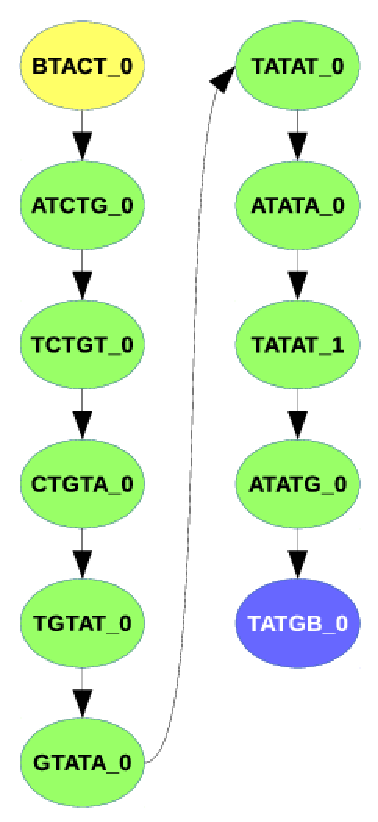
\includegraphics{img/ref-my.pdf}
	\caption{Graph resulting from the transformation of \texttt{ATCTGTATATATG} sequence}
	\label{fig:ref-my}
\end{figure}

\begin{figure}
	\centering
	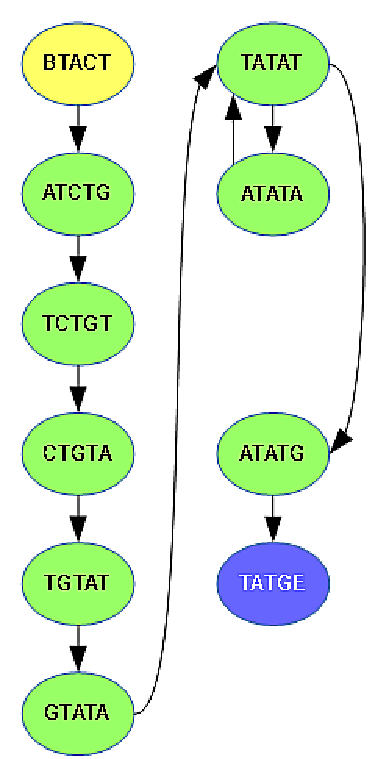
\includegraphics{img/ref-db.pdf}
	\caption{Transformation of the ATCTGTATATATG squence to a standard De Bruin graph (with no k-mer context numbers)}
	\label{fig:ref-db}
\end{figure}

Although we solved the loop problem, for now, by not allowing them to appear, and thus making the graph, at this stage, linear, things get more complicated in the next step that covers introducing individual reads into the graph.

\section{Adding Reads}

Basic idea behind this step is farily simple and similar to the approach used in the previous one. The read being added is divided into a sequence of k-mers. If a k-mer is not represented by any existing graph vertex, a new vertex is created for it. In other cases, existing vertices are used. Again, vertices representing adjacent k-mers in the read are connected by edges. 

\subsection{The Idea}
\label{subsec:idea}

Figure \ref{fig:read-idea} shows a graph created by transforming a region of \texttt{ACCGTGGTAAT} and adding a read \texttt{ACCGTAGTAAT} to the resulting graph. The read is divided into the following k-mers
\begin{gather}
k_0 = ((A, C, C, G, T), 0) \\
k_1 = ((C, C, G, T, A), 0) \\
k_2 = ((C, G, T, A, G), 0) \\
k_3 = ((G, T, A, G, T), 0) \\
k_4 = (T, A, G, T, A), 0) \\
 k_5 = ((A, G, T, A, A), 0) \\
k_6 = ((G, T, A, A, T), 0)
\end{gather}

In the graph, there already are vertices representing k-mers $k_0$ and $k_6$. For other others, new vertices are created. Finally, edges are added (if necessary) to show the k-mers order within the read. The figure also suggests how to retrieve the sequence covered by the read – just by following the edges and using the last base of all the k-mers except the first one. 

Figure \ref{fig:read-idea} reflects an ideal state, meaning that all places where the read differs from the reference are covered by distinct k-mers, and distance between each two of them is greater than $k$. If these conditions are met, each single $n$-base long difference (SNP, insertion or deletion) adds exactly $k$ new vertices to the graph. However, it may happen that some of the k-mers covering a difference colide by sequence with either k-mers of the reference, or k-mers of other reads covering totally different place of the active region. To minimize such unfortunate cases, additional graph transformations need to be made after all the reads are added to the graph.

\begin{figure}
	\centering
	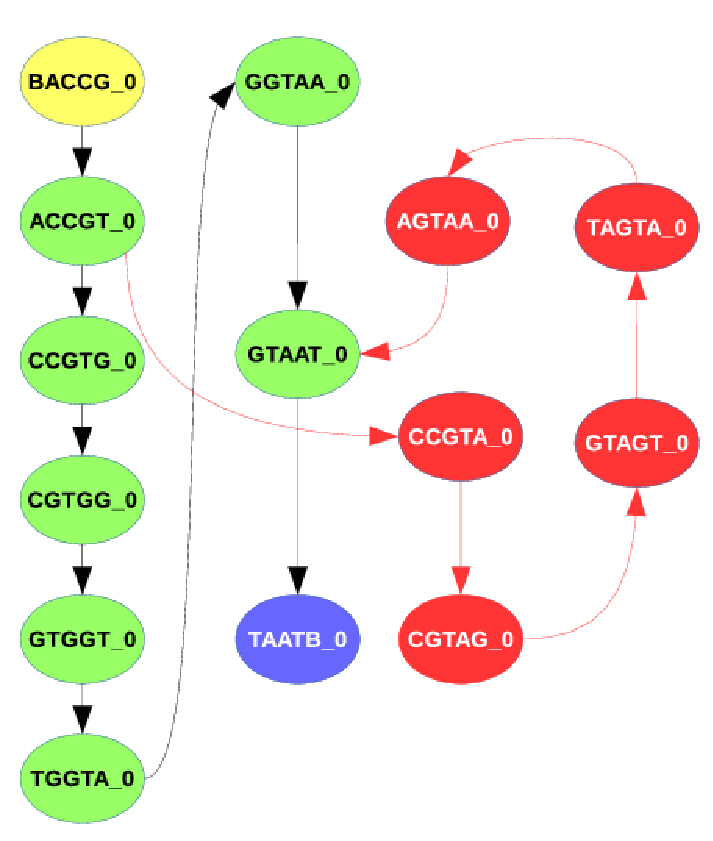
\includegraphics{img/read-idea.pdf}
	\caption{Basic idea behind adding a read into a De Bruin graph}
	\label{fig:read-idea}
\end{figure}

Unfortunately, this idea does not work in our case. Introduction of the k-mer context numbers prevented loops in the graph derived from the reference. But since multiple k-mers representing the same sequence may exist, it is not always possible to easily determine which of the vertices should be assigned to individual k-mers of the read. For example, if looking at the graph from Figure \ref{fig:ref-my}, it is not clear which vertex (or vertices) should be assigned to a k-mer with \texttt{TATAT} sequence. 

We decided to solve the issue by transforming the basic idea into the following steps:
\begin{itemize}
\item divide the read into sequence of k-mers (a short variant optimization may be applied),
\item assign a set of vertices to each k-mer, so that all vertices in the set represent k-mers euqal to the read k-mer by sequence,
\item from each set, select a vertex to represent the k-mer of the read,
\item connect the vertices representing the read to respect the order of the k-mers in the read.
\end{itemize}

\subsection{Transforming the Read into K-mers}

Let's define a read of length $n$ as a sequence $(r_0, ..., r_n)$ of bases. If the short variant optimization is not applied, the sequence is divided into individual k-mers $k_0, ..., k_n-k$ in the same way as for the reference case, except that no extra k-mers are created. They look as follows:
\begin{gather}
k_0 = ((r_0, ..., r_k-1), 0) \\
... \\
k_{n-k} = ((r_{n_k}, ..., r_{n-1}), 0)
\end{gather}

Then, the next step is applied (\ref{subsec:assign-sets}).

As described in \ref{subsec:idea}, in an ideal case, an $n$ base long difference from the reference produces $n + k - 1$ k-mers different from all reference k-mers. To reduce the probablity taht some of the k-mers actually colides with either the reference, or another read, the short variant optimization may be applied. The optimization reduces the number of k-mers representing to:
\begin{itemize}
\item $n$ for for an insertion,
\item zero for a deletion,
\item $1$ for a SNP.
\end{itemize}

The optimization assumes that when recovering a sequence from the graph, only the last base of each k-mer, wth an exception of the starting one, is used. So, only k-mers covering the difference by their last base need to be added; reference k-mers may be used for the rest in case the difference is followed by some number of bases equal to the reference. 

Figure \ref{fig:read-optimization} shows how the graph is optimized for a read containing SNP. The reference and read sequences are taken from Figure \ref{read-idea}. Since, the difference has 1 base in length, only one k-mer (\texttt{CCTGA\_0}) is used to represent it. The k-mer is followed by reference k-mers. As can be seen, their last base is equal to one of k-mers from Figure \ref{read-idea}.

\begin{figure}
	\centering
	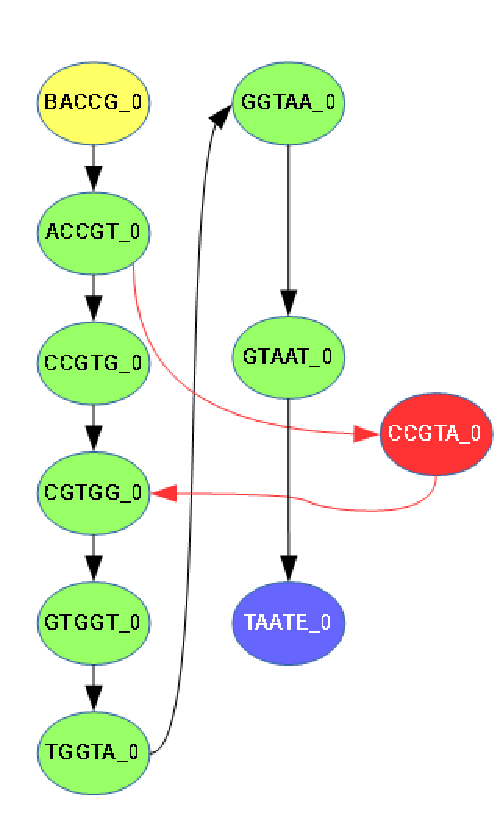
\includegraphics{img/read-optimization.pdf}
	\caption{Short Variant optimization}
	\label{fig:read-optimization}
\end{figure}

The short variant optimization is applied for k-mer $k_i$ if the following holds:
\begin{itemize}
\item There is only one vertex $v_{Ref_{j-1}}$ for $k_{i-1}$ and that vertex was added during the reference transformation phase,
\item There is at most one vertex for $k_i$ that either is a result of a read addition, or is a reference one but do not immediately follows  $v_{Ref_{j-1}}$ in the reference.

Such conditions are met when the read differs from the reference at base $r_{i+k-1}$. To determine whether the difference is only a short one, the Smith-Waterman algorithm is applied. If this is the case, the action depends on the difference type:
\begin{itemize}
\item for deletion, $k_i$ is defined as $v_{Ref_{j + n - 1}}$,
\item for insertion, $k_i$, ..., $k_{i + n - 1}$ are defined as with no short variant optimization and $k_{i + n}$ is set to $V_{Ref_{j}}$,
\item for SNP, $k_i$ is left as such and $k_{i+1}$ is defined as $V_{Ref_{j+1}}$
\end{itemize}
\end{itemize}

\subsection{Assigning Sets of Vertices to K-mers}
\label{subsec:assign-sets}

The process of assigning vertex sets to individual k-mers derived from the read in the previous step is quite straightforward – a set assigned to certain k-mer contains exactly the vertices representing k-mers with sequence equal to the k-mer. The k-mer context number is not taken into account. If a k-mer is not represented by any vertex of the current graph (thus, the k-mer would receive an empty set), a new vertex is created to represent it.

Previous steps of the algorithm, described above, impose the following conditions on the assigned vertex sets:
\begin{itemize}
\item each set contains either read, or reference vertices, not both,
\item if a set contains read vertices, its size is always one,
\item sets containing reference vertices do not have such restriction,
\item each two sets are either distinct (their intersection is an empty set) or equal.
\end{itemize}
The second and third condition holds because k-mer context numbers are used to differentiate reference k-mers but not the read ones. 

In formal terms, a set $M_i$ is assigned to a k-mer $k_i$ where
$$
M_i = {v_{i_j} | v_{i_j} \in V(G), kmer(v_{i_j}) equals to k_i by sequence}
$$ 
When a set is assigned to each k-mer, it is time to integrate the read into the graph in form of a path, starting on a vertex representing $k_0$ and ending in one covering $k_{n-k}$. SInce $M_i$ sets may contain more than one vertex, it is required to select vertices to form a path best fitting to the read. To derive a good path, we decided to the following observations about reads:
\begin{itemize}
\item they should follow the reference sequence in a forward direction,
\item probability of making big leaps in that direction is low,
\item multiple reads cover one place, thus sharing appropriate parts of their paths.
\end{itemize}

These observations cannot be enforced too strictly because De Bruin graphs are not very suitable for coping with repeats of length $k$ or more, and similar phenomenoms. The case of a read containing a copy of reference at leat $k$ baes in length might be enough to break the first observation. The second observation permits exceptions by definition. The third one, forms a base for most of the genome assembly algorithms.

To solve the problem of selection of the right vertices from the $M_i$ sets, we decided to reduce it to a shortest-path problem on a helper graph the structure of which is defined by the sets and their contents.

\subsection{The Helper Graph}
\label{subsec:helper-graph}

The helper graph is an oriented layered one. Each layer consists ofall vertices  vertices contained in one reference $M_i$ sets. The order of the layers respect the order of $M_i$ sets. Sets consisting of read vertices are not part of the helper graph. Ony adjacent layers are connected by edges, their orientation reflects the order of the sets. Each subgraph consisting of two adjacent layers is a full bipartite graph. The structure of the helper graph does not take equality of $M_i$ into account. In other words, when $M_i = M_j$ for $i \ne j$, both sets are represented within the heper graph as individual layers, even if they refer to the same vertices of the (main, non-helper) graph.

Formaly speaking, let $M_i = \{v_{i}^{1}, ..., v_{i}^{n_i}\}$ and let $i$ serves as an index to reference sets only. Then the heper graph $G_h$ can be defined as follows:
\begin{gather}
G_h = (V_h, E_h) \\
V_h = \cup_i M_i \\
E_h = \{(u, v) | u \in M_i, v \in M_{i + 1}\}
\end{gather}

By finding the shortest path leading from a vertex in the first layer to one in the last layer, we perfrom the process of selection of vertices to represent the read in the main graph. The shortest path depends on weights of edges connecting the adjacent layers of the helper graph. In general, the weighting funcgion follows these rules:
\begin{itemize}
\item the weight is increased by a \textit{missing edge penalty} if there is a missing edge on the path from $u$ to $v$ in the main graph,
\item the weight is increased by a \textit{reference backward penalty} if reference position of $u$ is greater or equal to the reference position of $v$,
\item the weight is increased by a \textit{reference forward penalty} if reference psotiion of $u$ is far less than reference position of $v$.
\end{itemize}
The rules actually indicate why $M_i$ sets covering read vertices are not parts of the helper graph – since their vertices maintain no reference position, only the missing edge penalties applies and that can be included within missing edge penalties of the reference vertices only.

For an example of a helper graph, let's have a reference sequence \texttt{ACTATACTA} and a read \texttt{ACTAGACTA}. The left part of Figure \ref{fig:heper-graph-short} shows the main graph just after adding vertices for the reference and the read k-mers with short variant optimization applied. The resulting helper graph is shown on the right part of the figure.

Six k-mers are derived from the read which means that vertex sets $M_0$, ..., $M_5$ are assigned to them. Since the second k-mer is represented by a read vertex, the $M_1$ set is not included as a layer of the helper graph. Other sets contains reference vertices, so they form individual layers. Adjacent layers are then connected. Edges with applied penalties (only the reference backward penalty in this case) are depicted red. The black edges show the shortest path.

The shortest path select the first vertex from $M_0$ and the second one from $M_5$ to represent the read within the main graph (since other sets contain only one vertex, the selection process is trivial there). The resulting path in the graph can be used to correctly recover the sequence covered by the read.

\begin{figure}
	\centering
	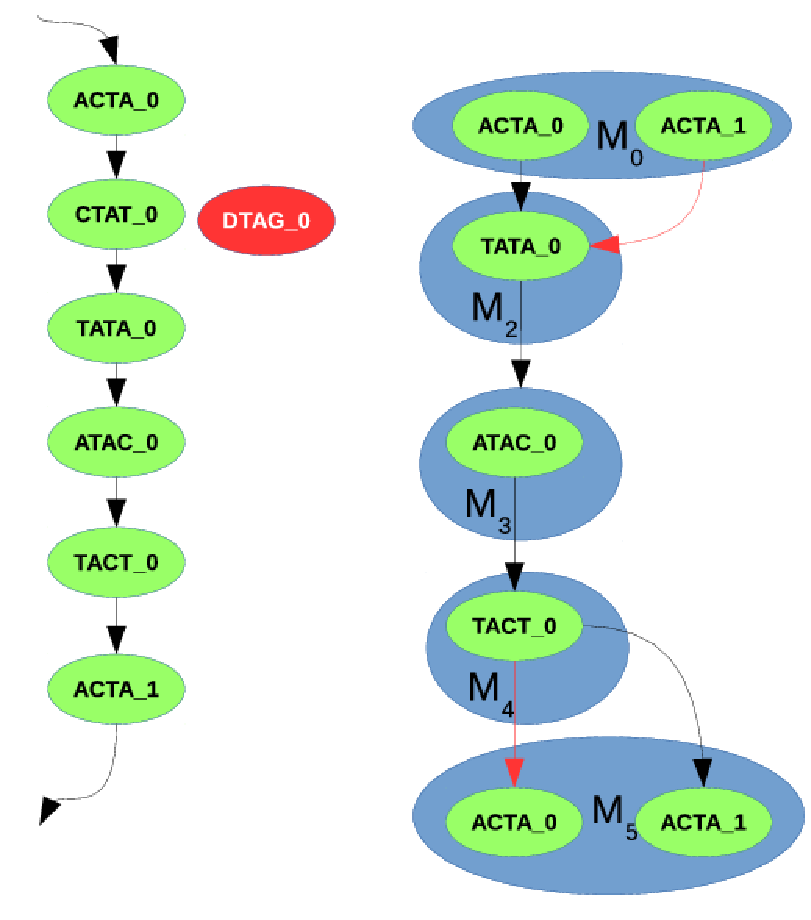
\includegraphics{img/helper-graph-short.pdf}
	\caption{Helper graph creation with short variant optimization}
	\label{fig:helper-graph-short}
\end{figure}

As Figure \ref{fig:helper-graph} indicates, both graphs look a little bit differently when the short variant optimization is not applied. The main graph contains more read vertices which reduces the number of layers in the helper graph. Although the graphs are different, the sequence covered by the rad is the same and can be correctly recovered again.

\begin{figure}
	\centering
	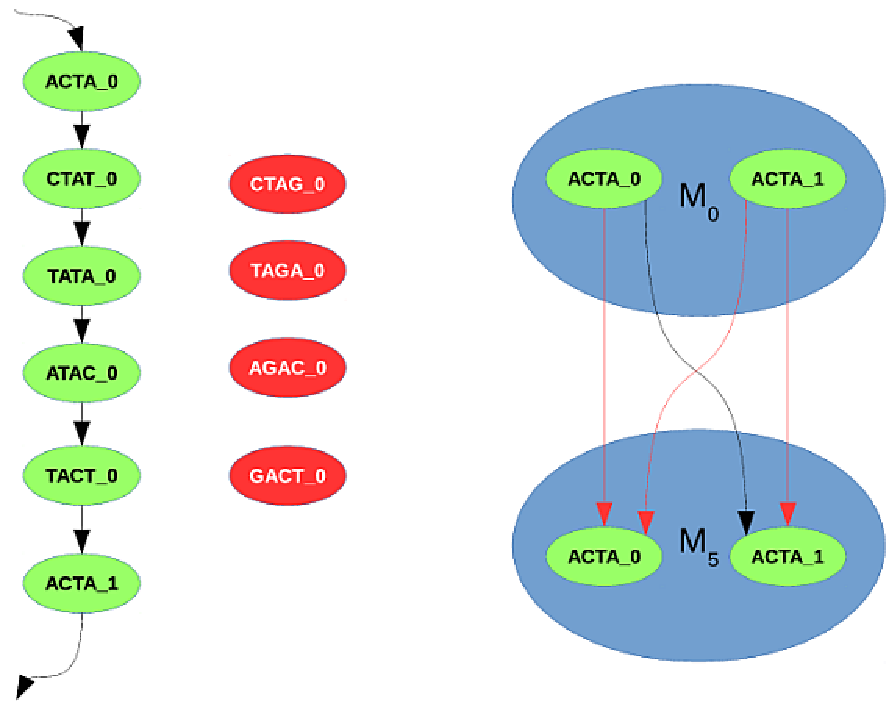
\includegraphics{img/helper-graph.pdf}
	\caption{Helper graph creation without short variant optimization}
	\label{fig:helper-graph}
\end{figure}

\section{Graph Structure Optimization}
\label{sec:graph-structure-optimization}

When all reads are integrated into the De Bruin graph, it is time to optimize its structure in order to get rid of unpopulated paths, usually created by read errors, and resolve some other issues caused mostly by repetitive regions inside either the reference or the reads.

\subsection{Connecting Bubbles}
\label{subsec:connecting-bubbles}

Figure \ref{fig:bubble-connection} demonstrates one class of the structural problems. A subset of reference sequence was transformed into vertices 1, 2, 3, 4, 5 and 6. A set of reads is represented by a "path" 2, 3, 4, 5, R1, R2, 1, 2, 3, R3, 6.  The left part of the figure shows how such a graph woud look like without any optimizations. It is clear that recovering the correct sequence would not be trivial. 

Howerver, since we know that the path leads from R2 to R3 (through 1, 2, 3), we can theoretically replace edges (R2, 1) and (3, R3) by a special edge (R2, R3), as the right part of the figure suggests. An information about the sequence covered by vertices 1 and 2 needs to be recored within the new edge. Recovering the correct sequence from the right part of the figure does not impose a problem since it is just a simple bubble. 

\begin{figure}
	\centering
	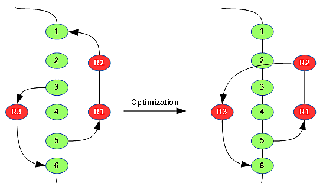
\includegraphics{img/bubble-connection.pdf}
	\caption{Benefits of connecting bubbles}
	\label{fig:bubble-connection}
\end{figure}

